
\ifx\headerIncludedJR\undefined
  \documentclass[11pt,a4paper]{article}
  \setlength{\textwidth}{5.50in}
  \usepackage[utf8]{inputenc}
\usepackage[T1]{fontenc}
\usepackage{amsmath}
\usepackage{amsthm}
\usepackage{amssymb}
%\usepackage{rotating}
%\usepackage{amslatex}
\usepackage{siunitx}
\usepackage{multicol}%for multicol
\usepackage{blkarray}%blockarray and block
\usepackage{comment}
\usepackage{fnbreak}%get a warning if a footnote is split
\usepackage[section]{placeins}
\usepackage{listings}
\lstset{breaklines=true,basicstyle=\ttfamily,language=Python}
\usepackage{arrayjobx}
\usepackage{array}%for \newcolumntype
%\usepackage[shortlabels]{enumitem}
\usepackage{mathtools}
\usepackage{afterpage}
\usepackage{setspace}% for \setstretch
\usepackage{algorithm}
\usepackage{algpseudocode}%for algorithmic
\usepackage{thmtools}%so that autoref works with Lemmas
\usepackage{tikz}
\usepackage{pgfplots}
\pgfplotsset{compat=1.15}
\usepackage{shuffle}
\usepackage{textcomp}%for \textrecipe
\usepackage{fontawesome}%for \faTable
\usetikzlibrary{calc,shapes,arrows.meta,decorations.markings,arrows}
\usetikzlibrary{graphs,positioning,svg.path,backgrounds}
\newcommand{\tikzmark}[1]{\tikz[overlay,remember picture] \node (#1) {};}
%\usepackage{CJKutf8}%for CJKChar

%\usepackage[backend=biber,backref=true]{biblatex}
\usepackage[backend=biber,style=alphabetic,backref=true,maxbibnames=10]{biblatex}
\addbibresource{sigs.bib}
\usepackage{url}

\usepackage{imakeidx}
%not a list of definitions, just symbols and abbreviations
%What is an abbreviation? Is QR? 
\makeindex[intoc,title=Symbols and abbreviations index]
\def\jind#1{\index{#1}}
\def\jindmath#1#2{\index{#2@$#1$}}
\def\jindv#1{\index{#1v@\texttt{#1}}}
%Some places I've given up and used \index in the text 
\definecolor{bluee}{rgb}{0.4, 0.4, 1.0}
%https://tex.stackexchange.com/questions/134191/line-breaks-of-long-urls-in-biblatex-bibliography
\setcounter{biburlucpenalty}{8000}
\setcounter{biburllcpenalty}{8000}

\usepackage{hyperref}

%so that autoref works with algorithms
\newcommand{\algorithmautorefname}{Algorithm}

%might help url breaking in bibliography
%\Urlmuskip=0mu plus 1mu minus 1mu
%also all the emergencystretch/looseness/fussy/sloppy
%to play with
%https://tex.stackexchange.com/questions/18505/how-to-use-sloppy-for-just-some-references

\def\ii{{\texttt{iisignature}}}
\def\pypi{{\texttt{PyPI}}}
\def\numpy{{\texttt{numpy}}}
\def\scipy{{\texttt{scipy}}}
\def\i#1{\index{#1@\texttt{#1}}}
\def \hilite#1{\underline{\color{blue}\textbf{#1}}}
%\def \alph#1{{\color{blue}\mathbf{#1}}}
\def \lex{<_L}
\def\kron{\underline{\otimes}}

\graphicspath{{C:/Users/Jeremy/Dropbox/phd/graphs/}{/home/jeremyr/Dropbox/phd/graphs/}{/Users/reizenstein/DropboxPersonalSymlink/phd/graphs/}}

%\RequirePackage{relsize}
%\DeclareRobustCommand\CXX{C\kern-.05em \raisebox{.3ex}{\scalebox{0.9}{\textbf{+\kern-.10em+}}}}
\DeclareRobustCommand\CXX{C\kern-.05em {\scalebox{0.9}{\textbf{+\kern-.10em+}}}}
%\DeclareRobustCommand\{\texorpdfstring{\CXX}{C++}}
\DeclareRobustCommand\CC{C\texttt{++}}
\def\bftab{\fontseries{b}\selectfont}
\newtheorem{theorem}{Theorem}
%\newtheorem*{theorem*}{Theorem}%bad idea, because you can't refer to it.
\newtheorem{definition}[theorem]{Definition}
%\newtheorem{outsideTheorem}[theorem]{Theorem}
\newtheorem{example}[theorem]{Example}
\newtheorem{conjecture}[theorem]{Conjecture}
\newtheorem{lemma}[theorem]{Lemma}
\newtheorem{proposition}[theorem]{Proposition}
\newtheorem{remark}[theorem]{Remark}

\newcommand{\area}{\mathsf{area}}
\newcommand{\Area}{\mathsf{Area}}
\newcommand{\emptyword}{\epsilon}
\newcommand{\ds}{d} % dimension of the signal
\newcommand{\TC}{T((\R^\ds))} % concat
\newcommand{\TS}{T(\R^\ds)} % shuffle
\newcommand{\GL}{\operatorname{GL}}
\newcommand{\SO}{\operatorname{SO}}
%\newcommand{\id}{\operatorname{id}}
\newcommand{\id}{\mathsf{id}}

\newcommand{\evaluatedAt}[1]{\,\raisebox{-.5em}{$\vert_{#1}$}}

\def\hssymbol{\mathbin{\succ}}
\def\hs#1#2{#1\hssymbol#2} %half shuffle
%\def\hs#1#2{z(#1,#2)} %half shuffle
\def\areab#1{\underline{\area}(#1)}
\def\areabb{\underline{\area}}
\newcommand{\R}{\mathbb{R}}
\newcommand{\Q}{\mathbb{Q}}
\newcommand{\C}{\mathbb{C}}
\newcommand{\N}{\mathbb{N}}
\newcommand{\spann}{\operatorname{span}}
\newcommand{\sign}{\operatorname{sign}}

\DeclareMathOperator*{\argmax}{arg\,max}
\DeclareMathOperator*{\argmin}{arg\,min}
\DeclareMathOperator{\softmax}{softmax}

%indicate that this file has been had
\def\headerIncludedJR{}
\def\endDocumentJR{}

%general hints
%https://homepages.inf.ed.ac.uk/imurray2/compnotes/latex.html

  %this cannot be in header.tex as it messes up
  %the thesis copyright page
  \def \alph#1{{\color{bluee}\mathbf{#1}}}
  \begin{document}
  \tableofcontents
  \def\endDocumentJR{\printindex \printbibliography[heading=bibintoc]\end{document}}
\fi

\section{Introduction}
\def\parameterSize{\scriptsize}
\label{sec:dlintro}
The Chinese and Japanese  languages are very popular and have similar writing systems.
%Vietnamese no more
%Korea: chinese chars (Hanja) only replace the simple Hangul alphabet a little bit in South Korea
With the widespread use of smartphones and touch devices in the last decade, automated recognition is relevant to allow text input via letter drawing rather than by keyboard, which can be inefficient.
The leading mobile operating systems, Apple's iOS and Google's Android, provide built-in handwritten input, and third-party apps are also available.
Mobile devices have limited compute power because of battery life. Therefore computationally efficient methods are important.

There is a long history of methods for handwritten Chinese character recognition. 
Much of the work has treated the case of recognising the input from an image, for example of a paper manuscript.
This is termed \emph{offline} character recognition, and is distinguished from \emph{online} character recognition where the data is given as a sequence of strokes with their points supplied in order. The order and directions of the strokes is potentially useful, so better accuracy is potentially possible in the online setting by exploiting the extra information available. The online problem is the relevant one for handwriting interfaces on devices.

When I started looking at this problem in 2014, there were a number of methods for performing online Chinese recognition, each with some pros and cons.
The first promising method used an 8x8 spatial grid of 8-directional histograms \cite{histograms}. The approach showed the importance of capturing both the location of the pen, and the direction of the pen's movements. The method is computationally fairly cheap, but the accuracy was limited. Ad hoc pre-processing was needed to reshape the characters to deal with the lack of awareness of translation invariance of human handwriting. 
%Given a circle, there would be a large in calculating the radius, for example.
Given a circle, there is a large margin of error if you try to calculate the radius from the 8x8x8 histogram due to the coarse resolution of the 8x8 spatial grid.
%It is hard to tell the difference between a small circle and a larger circle due to the low resolution.

From around 2010, the most successful methods were using large convolutional neural networks. They capture the identity and shape of each stroke separately, together with order.  The winner of the Chinese Handwriting Recognition Contest 2010 \cite{chinese2010} with 92.39\% accuracy (on the same data as we use) used histogram features along with such a large network.

Schmidhuber and collaborators \cite{multicolumn} used a higher resolution convolutional network which was therefore more computationally expensive, achieving greater accuracy (94.39\%). %same data
This was not using signatures
%had been achieved earlier with a more computationally expensive model, not using signatures.

Combining convolutional networks with signatures boosted accuracy but the computational cost was still rather high
-- 96.18\% accuracy by Ben Graham in \cite{BEN} was the best in the ICDAR 2013 Chinese
Handwriting Recognition Competition \cite{chinese2013}.

%GPEN … mobile phones .. want a computationally cheap solution …
One of the leading third-party apps is GPEN \cite{GPEN} from the South China University of Technology, one of their papers from a bit later is \cite{Improved}. They use
signature features as part of the representation, and also a large convolutional network. In such apps reducing the required power for classification is always a priority, although efficient training is also attractive.

Recurrent neural networks, such as LSTMs, offer an alternative way to learn sequence data which can be fast compared with convolutional networks. 
Combining LSTM with signatures was an attractive idea to us as the signatures would capture local shape information potentially very cheaply, allowing the deep learning problem of combining the partial signatures to be relatively small, and so we wanted to investigate this possibility.  We constrain ourselves to working with the raw data, as we wish to develop algorithms that can generalise well, rather than needing human-intensive problem specific work on feature engineering which requires much trial and error. The test set only has 60 writers, and much of the test error is concentrated on a few of them. There is a danger that feature engineering results in methods that work well on the test set, but does not generalise well to writers outside the dataset. 

An example of LSTM with feature engineering and customised data augmentation is \cite{BengioChinese1} which first appeared on ArXiv in June 2016 and then showed the best accuracy yet, albeit using an enlarged training set. It shows LSTM is a good fit for the problem domain, but powerful universal local shape characterisation is desirable.

\iffalse
The first promising method used an 8x8x8 grid of directional histograms \cite{histograms}, which is computationally cheap. It doesn't capture the curvature of each stroke in a simple way. It showed that the direction is important above location of strokes.

We want to capture the identity and shape of each stroke separately, together with order.

When I started looking at this in 2014, the implemented models and the best published models, as far as I can tell, used large convolutional neural networks. One of the leading third-party apps is GPEN \cite{GPEN} from the South China University of Technology, one of their papers from the time is \cite{Improved}. They use signature features as part of the representation.
Great accuracy (94.39\% on the same data as us) had been achieved earlier with a more computationally expensive model, not using signatures, in \cite{multicolumn}.
Ben Graham had used a large convolutional network together with signatures to get 96.18\% accuracy in \cite{BEN} which was the best in the ICDAR 2013 Chinese Handwriting Recognition Competition \cite{chinese2013}.
%Lower accuracy and cheaper computation has been around for a long time by using grids of histograms as features, for example in \cite{histograms}, and such features were involved in the best results before 2012, namely the winner of the Chinese Handwriting Recognition Contest 2010 \cite{chinese2010} with 92.39\% accuracy.

Since I started, there has been significant other progress which shows that a single recurrent network can learn both faster and more accurately than previous techniques. Signatures are not involved. The first paper was \cite{BengioChinese1} which appeared first in June 2016 on ArXiv.
Recurrent networks can become slow when the input data has a very long time dimension or there are many hidden units.
\fi

Here, I will introduce some background to the problem and deep learning methods in general, and show a potential pipeline for using signatures in combination with recurrent neural networks.
%I am more interested in the mathematically motivated improvements to a pipeline than fine-tuning a method, which requires much more parameter exploration and care with feature engineering and data augmentation.

\section{Description of data}
The CASIA datasets \cite{CASIA} are large standard datasets for Chinese handwriting recognition. The task we are attempting is the online character recognition problem. We pick one of the standard databases for the task, namely the online handwritten character database 1.1 (\verb|OLHWDB1.1|).% and use it with its normal train-test split.
\footnote{Another suggested procedure, for example used in \cite{BengioChinese1}, is to combine data from both the 1.0 and 1.1 datasets. This is actually recommended in \cite{CASIA}.}
There are samples of 3755 different characters (both symbols and Chinese characters) written by 300 different writers with a special \emph{Anoto} pen which records each stroke as a sequence of coordinates. 
This data is directly comparable to data from a touch interface.
We split them in the standard recommended train-test split, so that the first 240 writers' data is used for training and the last 60 for testing. The data in total consists of 939,564 labelled sample characters for training and 234,800 for testing. The order of writers is random, so both the training set and the testing set should be representative of the pool of writers. (This is not true in the 1.0 database).
On average, a character has 5.6 strokes, with the maximum number in a character being 26. On average, a character is described by a total of 60.9 points, with the maximum being 283. A stroke is described by on average 10.9 points, with the maximum being 192.
\autoref{fig:chineseDemo} shows some examples of three characters from the training set. A Chinese native described the handwriting to me as bad but readable.
%Our db has 898110 characters for training, not 939564. For testing, we have 224442 not 234880
%Total number of strokes for training is 4996380
%Max # strokes in character is 26 %select max(b) from (select count(*) as b from strokes group by trainxn)
%min is 1
%max length of a stroke is 192 %select max(length(data))/8 from strokes;
%min is 1
%max #points in a stroke is 283 %select max(b) from (select sum(length(data)) as b from strokes group by trainxn)
%total #points is 54678864
%average #points in a stroke is 10.9
%average #points in a character is 60.9
%average #strokes in a character is 5.6
\begin{figure}
%\begin{center}
\centering
  \includegraphics[width=3.487in]{chineseDemo}
  \caption[Example Chinese characters from the CASIA \texttt{OLHWDB1.1} training set.]{Three Chinese characters and their handwritten versions as provided by each of the first four writers in the CASIA \texttt{OLHWDB1.1} training set. Note that the number of strokes in a single character can vary between writers. (These are Unicode code points \texttt{0x997a}, \texttt{0x7f34} and \texttt{0x7ede}.) }
  \label{fig:chineseDemo}
%\end{center}
\end{figure}

\section{Generic supervised learning setup}
The typical setup in supervised machine learning is %as follows. 
that
we want to learn an unknown function $f$ from training example space $X$ to output space $Y$.
We are given a \emph{training set} of examples from $X$ for which $f(X)$ is known. 
\subsection{Augmenting the output space}
Often the output of a network needs to be a probability distribution rather than discrete values, and we define a loss function to optimise.
We define a possibly augmented output space $\hat Y$ which is continuous and for which there is a simple deterministic function $i:\hat Y\twoheadrightarrow Y$. 
We also define a cost function $c:Y\times\hat Y\to \mathbb{R}^+_0$ 
where a high value of $c(y,\hat y)$ indicates that the prediction $\hat y\in \hat Y$ is bad when the right answer is $y$.

We make some form of a model, a function $\tilde f$, which takes a sample $x\in X$ and set of parameters $\lambda$ in parameter space $\Lambda$ to the constructed output space $\hat Y$. The aim of training is to come up with a $\lambda\in\Lambda$ such that for a sample $x$, $i(\tilde f(x,\lambda))$ is roughly $f(x)$. 

We pick $\hat Y$, $i$, and $c$ in conjunction with the model so that changing $\lambda$ to reduce $c(f(x),\tilde f(x,\lambda))$ makes $i(\tilde f(x,\lambda))$ a good approximation of $f(x)$ and also so that $c(f(x),\tilde f(x,\lambda))$ is a differentiable function of $\lambda$.
In practice, $\tilde f$ is not only differentiable but its derivative is also easy to calculate, via the chain rule, in the form of autodifferentiation and the method of backpropagation of derivatives, as mentioned in \autoref{sec:backprop}.
If our formalism didn't allow for $\hat Y\ne Y$ then we would have a problem with allowing our cost to be differentiable with respect to the parameters if $Y$ was a discrete space.

For example, if you were training a model to distinguish pictures of cats from pictures of dogs, $Y$ would naturally be the set $\{\mathrm{dog},\mathrm{cat}\}$. In this case a sensible choice would be as follows.
\begin{align*}
\hat Y&=[0,1]
\\i(\hat y)&=\begin{cases}\mathrm{dog}&\hat y\le0.5\\\mathrm{cat}&\hat y>0.5\end{cases}
%\\j(y)&=\begin{cases}0&y=\mathrm{dog}\\1&y=\mathrm{cat}\end{cases}
\\c(y,\hat y)&=\begin{cases}-\log\hat y&y=\mathrm{dog}\\-\log(1-\hat y)&y=\mathrm{cat}\end{cases}
\end{align*}
The intuition here is that we make an element of augmented output space be a probability that a picture is a cat. The amount by which we are wrong, our cost, is the cross entropy between the true answer and the predicted answer.

If there are $k>2$ categories, we might choose the following, a one-hot encoding of the output:
\begin{align*}
Y&=\{1,\dots,k\}\qquad\text{say,}
\\\hat Y&=\mathbb{R}^k
\\i(\hat y)&=\argmax_{m\in \{1,\dots,k\}}(\hat y)_m
%\\j(y)_m&=\begin{cases}1&m=y\\0&m!=y\end{cases}
%\qquad\text{this function $j$ is called \emph{one hot encoding}}
\\c(y,\hat y)&=-\log(\softmax(\hat y)_y)
\intertext{where $\softmax:\hat Y\to\hat Y$ given by}
\softmax(\hat y)_m&=\frac{\exp(\hat y_m)}{\sum_{m'\in \{1,\dots,k\}}\exp(\hat y_{m'})}
\end{align*} is a smooth function which maps vectors to the standard simplex $\Delta^{k-1}$, i.e.~discrete probability distributions. $c$ is the cross-entropy of this distribution, or the negative-log likelihood of the model on the data.

As another example, we might be trying to learn a function whose image is $[0,1]$. In this case, we have no need for augmentation and a sensible choice might be as follows:
\begin{align*}
\hat Y&=Y=[0,1]
\\i(\hat y) &=\hat y
%\\j(y)&=y
\\c(y,\hat y)&=(\hat y-y)^2
\end{align*}
The cost function is the square of the $L^2$ norm. %Over all the data, the cost is \emph{mean squared error}.

\subsection{Minibatches and stochastic gradient descent}
\label{sec:minibatchesSGD}
With this setup, we can formulate training as a problem of stochastic gradient descent.
On a subset of $n$ of the training examples $\chi\in X^n$, the badness of some set of parameters $\lambda$ is given by 
\begin{align}
g_\chi(\lambda)=\sum_{x\in\chi}c(f(x),\tilde f(x,\lambda)).
\end{align}

One way to find the best parameters would be to set $\chi$ to the entire training set and numerically minimise $g_\chi(\lambda)$. We have first derivatives of $g_\chi$ so gradient descent would be a possibility. But $g_\chi$ would be very slow to calculate, as it would require passing over the whole dataset, and this would have to happen very many times.

We can think of $g_\chi(\lambda)$ as a random function as $\chi$ is uniformly distributed over some samples from the training data.
It is much more efficient to try to minimize this random function as a stochastic gradient descent. The typical procedure is to start by picking once some initial random parameters $\lambda$, then to repeat the following many times: pick a random subset $\chi$ of the training data, evaluate $g_\chi(\lambda)$ and $g_\chi'(\lambda)$, and update $\lambda$ using some ``stochastic gradient descent'' technique designed to minimise $g_\chi(\lambda)$.

The dimensionality of $\lambda$ can be large. Typically $\Lambda=\mathbb{R}^d$ for $d$ in the millions or billions.
It is generally not feasible to calculate or even store the second derivative 
$g_\chi''(\lambda)$ because it has $d^2$ elements.
Thus we cannot use minimisation techniques like Gauss-Newton or Levenberg-Marquardt which use the second derivative to determine the length of a step. $g_\chi'(\lambda)$ can give us an idea of a direction to move $\lambda$, but not an amount.
A simple minimisation technique which can work is to move a fixed amount (called the \emph{learning rate}) in a direction given by an exponentially weighted moving average of recently seen values of $-g_\chi'(\lambda)$.
This is called \emph{momentum}. There are a few other techniques which work well.
They have in common that the memory usage grows no more than linearly in $d$ and not at all in the number of steps of optimisation history available. 

\subsection{Inductive bias}
When choosing a supervised machine learning model, we are choosing what kinds of functions are relevant in trying to find one which agrees with our training data.
The \emph{inductive bias} is the set of built-in assumptions about functions to be considered which our choice implies.

\subsection{Invariants}
\label{sec:invariants}
Across supervised machine learning having more training examples enables building better models. 

If there are known symmetries, or approximate symmetries, in the domain of the function being learned, then it can make learning much more effective to take this into account. Only certain functions have any chance of being useful approximations of the target function $f$, those which are generally unaffected by the symmetry. If we have a true group of symmetries, where we know $f(s(x))=f(x)$ for all $s$ in some group of transformations, then we want $f$ to take a single value on each orbit. 
%We want the \emph{inductive bias} of our model to be appropriate.
Often the most effective way to take a symmetry into account is to restrict our model to a form of function which has (approximately) the desired symmetry, or which makes it easy to learn functions which have the desired symmetry.
For example, when learning a function on images we may use a convolutional neural network which often will return similar values under small translations of the input.
Similarly, when using a 1D convolutional neural network to classify a time series which I thought to be translation invariant (for example EEG voltage readings) I restricted the first convolutional layer to have multiplicative weights which sum to 0.
Significantly, the fact that the signature is invariant under reparametrisations of a path leads to its possible use as a source of features of paths in the common case that we know that reparametrisation should not matter.

\subsection{Data augmentation}
Often some symmetry or invariant in the domain cannot be built into the structure of the model, because it would be too complicated.
But the invariant still means that a single piece of labelled training data can count as more than one example, because some distortions of it is expected to be also a good training example.
Data augmentation in this way is an important part of making the most of a dataset.
For a given problem, we might establish a set of transforms under which our data would still be good, including the identity transform. When generating each training sample in each $\chi$, we put it through a randomly chosen transform.

For example, if you were training a simple convolutional neural network to distinguish pictures of cats from pictures of dogs, you might exploit the fact that a picture of an animal flipped along a vertical axis is a good synthetic example of a picture of that type of animal. 
Each training sample might be flipped with probability $\frac12$ before use in $\chi$.

There is ongoing research into good data augmentation transformations, for example \cite{AutoAugment}, and some Python libraries have been made available for images, for example \verb|Augmentor| and \verb|imgaug|.
Many of the same transformations used for images can be translated into path data, for example small rotations, shears and elastic distortions, although these libraries are not directly usable in our setting.

\section{Neural networks}
Neural networks (NNs), or artificial neural networks (ANNs), are a category of forms for $\tilde f$, our parameterised function which we want to find parameters for to make it solve a supervised learning problem. The function %$\tilde f$
is built from a series of layers, and each layer is made from ``cells'' or ``neurons'' in a manner analogous to the brain. \emph{Deep learning} is basically machine learning using neural networks.

\subsection{Fully connected}

The simplest neural networks are \emph{fully connected neural networks} (FCNNs)\jind{FCNN} or \emph{multilayer perceptrons} (MLPs).\jind{MLP}
A fully connected neural network looks like the following.
The input space, $X$ is $\mathbb{R}^{u_0}$ for some $u_0$.
The following must be given: a \emph{number of layers} $m$, a number of \emph{units} in each layer $(u_i)_{i=1}^m$, and a nonlinear function $\sigma:\mathbb{R}\to\mathbb{R}$ called the activation function.
The output space is $\hat Y=\mathbb{R}^{u_m}$.
Then an element $\lambda$ of parameter space is a sequence $(W_i,b_i)_{i=1}^m$ where each  $W_i$ is a real $u_{i-1}\times u_i$ matrix called the \emph{weights}, and each $b_i\in\mathbb{R}^{u_i}$ is a vector called the \emph{biases}.
If $x$ is a vector, matrix or array, I write $\sigma(x)$ for the result of applying $\sigma$ to $x$ elementwise.

The neural network is then the function $\tilde f=g_n$ defined as follows:
\begin{align}
  g_{0}(x,\lambda)&=x\\
  g_{i+1}(x,\lambda)&=\sigma(g_i(x,\lambda)W_i+b_i)
\end{align}

(There is a commonly encountered equivalent way to formulate this as follows. We have parameters $\lambda=(\tilde W_i)_{i=1}^m$ where each  $\tilde W_i$ is a real $(u_{i-1}+1)\times u_i$ matrix. Then we define
  \begin{align}
  g_{i+1}(x,\lambda)&=\sigma\Big(\begin{bmatrix}g_i(x,\lambda)\\1\end{bmatrix}\tilde W_i\Big).\qquad)%\text{)}
  \end{align}

There is lots of terminology. For $i>0$, an element in $g_{i}(x,\lambda)$ is said to be a \emph{neuron}, a \emph{feature}, a \emph{feature detector}, a \emph{cell} or a \emph{unit} or the activation of one. $g_i$ is the $i$th \emph{layer}.
Anthropomorphically, these values are thought of as the results of intermediate steps the network has learnt to calculate from the input on its way to the output.
The structure of a FCNN is unchanged if, as an extra first step, the input is multiplied by a fixed nonsingular matrix or a incremented by a fixed vector.
We might say the network ``sees'' its input as an element of affine space.

The most popular choice for $\sigma$ is called the \emph{rectifier}, $\sigma(x)=\max(x,0)$. We say such a network has \emph{rectified linear units} or \emph{ReLUs}, and hence may call $\sigma$ itself ``ReLU''. This and some other activation functions which are relevant later are plotted in \autoref{fig:activations}.
\begin{figure}
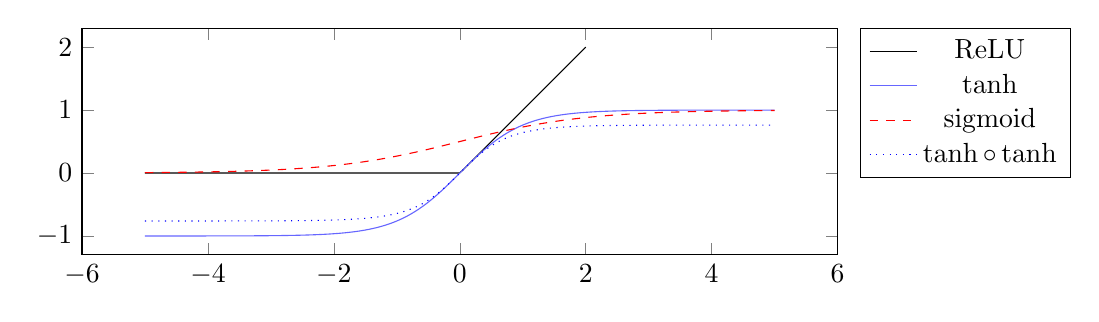
\begin{tikzpicture}
  \begin{axis}[
%    trig format plots=rad,
%    axis equal,
    axis equal image,
%    hide axis
%    thick, %affects border as well as plots
    width=0.8\textwidth, %even if the legend is outside, this only affects the axis object's scale, even though scale only axis is false (i.e. false means include just the axis labels etc)
    legend style={
      %legend pos=south east,
      legend pos=outer north east,
      %at={(0,-0.2)},
      %anchor=north west
    }
    ]
    \addplot [domain=-5:2, samples=200, black] {max(0,x)};\addlegendentry{ReLU}
    \addplot [domain=-5:5, samples=400, blue!60!] {tanh(x)};\addlegendentry{$\tanh$} %or semithick or something
    \addplot [domain=-5:5, samples=400, red, dashed] {1/(1+exp(-x))};\addlegendentry{sigmoid}
    \addplot [domain=-5:5, samples=200, blue, dotted] {tanh(tanh(x))};\addlegendentry{$\tanh\circ\tanh$}
  \end{axis}
\end{tikzpicture}

\caption{\label{fig:activations}Some important activation functions}
\end{figure}

\subsection{Convolutional}
Fully connected networks take their input to be $X=\mathbb{R}^{u_0}$ with no additional structure.
They know of no particular structure of the input space.
Often there is some structure which we want to be taken into account.
A common case is that we are given data in say $\mathbb{R}^{u_0^0}$ for each point on a lattice of shape $u_0^1\times u_0^2\times\dots\times u_0^d$.
Our data lives in the space $X=\mathbb{R}^{\prod_{i=0}^du_0^i}$.
Convolutional neural networks (CNNs\jind{CNN}) are a generalisation of fully connected neural networks which take this into account.
For example, if we are dealing with colour photographs of resolution $28\times28$ we would have $X=\mathbb{R}^{3\times28\times28}$, where we have a value for the brightness of red, green and blue at each pixel.
We want functions which treat pixels similarly to each other, and which treat neighbouring pixels similarly, to be favoured by the inductive bias of our model.
We want the model to be able to learn a function which doesn't change much if a picture is translated by about one pixel.

A convolutional network allows not just the input but other layers to have a grid structure.
The size of the array of values, or the number of units in layer $i$, $g_i(x,\lambda)$, is usually given by a sequence of numbers $u_i^0\times u_i^1\times\dots\times u_i^d$.
$u_i^0$ is known as the number of \emph{features} in the layer -- this is the number of values per point in space.
There are several common types of layers.
Two of the simplest are the convolutional and max pooling layers.
If layer $i+1$ is an $(l_1\times\dots\times l_d)$-\emph{convolutional layer} it contributes a vector $b_{i+1}\in\mathbb{R}^{u_{i+1}}$ and a (typically small) $u_{i}^{0}\times u_{i+1}\times l_1\times\dots\times l_d$-array $W_{i+1}$ to $\Lambda$.
Then, in a simple setup, the elements of the layer's outputs $g_{i+1}(x,\lambda)$ are the values of 
\begin{align}
  \sigma\Big(\sum_{j_0=0}^{u_{i}^0}\sum_{j_1=0}^{l_1}\cdots\sum_{j_d=0}^{l_d
 }(g_i(x,\lambda))_{(j_0,k_1+j_1,k_2+j_2,\dots,k_d+j_d)}(W_i)_{(j_0k_0j_1j_2\dots j_d)}+(b_i)_{k_0}\Big)
\end{align}
as $k_0$ ranges from 0 to $u_{i+1}^0$ and the other $k_p$ range from 0 to $u_{i+1}^p=1+u_i^{p}-l_p$.
There are numerous variations on this theme, for example treating the boundary differently or enforcing further sparsity on $W_{i+1}$.
The idea is that the new units at a point in space only depend on the values of the units in the previous layer near that point in space, and the manner of the dependence is the same over all space.
This layer is seen as analogous to the V1 cells in a visual cortex.
This is equivalent to a fully connected layer where the matrix $W$ is restricted to a very special sparsity pattern, and also that its nonzero values are repeated in a certain way.
% If layer $i+1$ is an $(l_1\times\dots\times l_d)$-\emph{max pooling layer}, then it contributes
A max pooling layer takes the maxima of each feature over a each of a grid of small cuboids which either cover each dimension or overlap in each dimension, thus preserving the number of features ($u_{i+1}^0=u_i^0$) but reducing the other dimensions.
It has no parameters. A typical such layer reduces the number of units in each spatial dimension by a factor of two.
The highest levels in a typical CNN typically take all the units to be a single vector and thus are fully connected, and so the output of the network happens in the same way as the FCNN\@.

\subsection{Recurrent neural networks}
The input being a sequence is an important case of a specially-structured input which it is important for the network to take into account.
A simple case is that for each example we are given data in say $\mathbb{R}^{u_0^0}$ for each of $u_0^1$ time points.
Our data lives in the space $X=\mathbb{R}^{u_0^0u_0^1}$.
We could be use a 1-D convolutional network (i.e.~one with $d=1$) in this case, but recurrent neural networks (RNNs\jind{RNN}) are an important alternative type of architecture in this case.
While convolutional and pooling layers allow the local spatial structure to be taken into account in the learning, RNNs force the temporal structure into the model, and explicitly globally, not just in a ``local'' way.
An RNN allows the network to allow earlier entries of the sequence to be taken into account when processing later entries.
Just like for fully connected and convolutional networks, the network is built from a sequence of layers.
The simplest RNN layer could take input as a sequence of $u_i^1$ values in $\mathbb{R}^{u_i^0}$ to output of the same number ($u_{i+1}^1=u_i^1$) of values in $\mathbb{R}^{u_{i+1}^0}$ % (with the time dimension unchanged )
Its parameters would be a weight matrix
 $u_{i-1}^0\times u_i^0$ matrix $W_i$, a second (square) weight matrix
 $u_i^0\times u_i^0$ matrix $\bar W_i$ for the recurrence, and a $u_i^0$-vector of biases $b_i$.
\begin{align}
  (g_{i+1}(x,\lambda))_1&=\sigma((g_i(x,\lambda))_1W_i+{}\phantom{(g_{i+1}(x,\lambda))_{t-1}\bar W_i+{}}b_i)\\
  (g_{i+1}(x,\lambda))_{\mathrlap{t}\phantom{1}}&=\sigma((g_i(x,\lambda))_{\mathrlap{t}\phantom{1}}W_i+           (g_{i+1}(x,\lambda))_{t-1}\bar W_i+b_i)&\text{for $t>1$}
\end{align}
(For a few paragraphs I am omitting the parameters $x$ and $\lambda$ from $g$).
Intuitively, what is happening here is that a learned map is converting a hidden state $(g_{i})_t$ to a new hidden state using one more piece of source data.
The hidden state can store a representation which knows about everything which has already been seen.

If we need to output one value for the whole sequence, the highest levels of the RNN will be fully connected, initialised from just the final timestep of the last recurrent layer, i.e.~$(g_{i})_{u_i^1}$.

\subsection{LSTM}
When trying to use RNNs when the sequence is long, it is hard for the early parts (low $t$) of the sequence to influence the final state, and thus there is a limit to what the network can learn.
The state has to be remembered through many multiplications by the matrix  $\bar W_i$.
For most values of $\bar W_i$ the derivative of $(g_i)_{u_i^1}$ with respect to an element in $(g_{i-1})_t$ for $t\ll u_u^1$ will be very large or very small.
This is called the problem of exploding or vanishing gradients.

% As a result, the network will not learn

Long-short term memory (LSTM, \cite{LSTM}\jind{LSTM}) is a variation of a recurrent layer which is designed to allow information to survive in the state across many timesteps.
There are two separate sets of units which operate in pairs.
To each output element $\big((g_i(x,\lambda))_{t}\big)_j$ is associated a memory cell
$(c_t)_j:=\big((c_i(x,\lambda))_{t}\big)_j$.
The layer needs parameters\footnote{Note that in this widely accepted notation, the \textbf{superscripts} $i$, $o$ and $f$ are decorations not variables nor placeholders.}
$u_{i-1}\times u_i$ matrices $W_i^f$, $W_i^i$, $W_i^o$ and $W_i^c$, $u_{i}\times u_i$ matrices $\bar W^f_i$, $\bar W^i_i$, $\bar W^o_i$ and $\bar W^c_i$, and
$u_i$-vectors $b_i^f$, $b_i^i$, $b_i^o$ and $b_i^c$.
The layer uses the sigmoid function, $\sigma'(x)=\frac1{1+e^{-x}}$ which is monotone increasing from $\mathbb{R}$ to the interval $(0,1)$. The normal activation function, $\sigma$, is usually $\tanh$.
They are evaluated for $t>1$ using temporary variables $f_t$, $i_t$, $o_t$ and $\tilde c_t$ as follows.
\begin{align}
  % trying to make everything line up exactly with phantoms/phanta is a bit of a pain here.
  % because W^f and W^{other letter} are lined up quite differently
\gdef\makevar#1{#1_t&=\sigma'((g_i(x,\lambda))_tW^{#1}_i+(g_{i+1}(x,\lambda))_{t-1}\bar W^{#1}_i+b_i^{#1})}  \makevar{f}\\
  \makevar{i}\\
  \makevar{o} \\
  \tilde c_t  &=\phantom{\sigma'}\mathllap{\sigma}((g_i(x,\lambda))_tW^{c}_i+(g_{i+1}(x,\lambda))_{t-1}\bar W^{c}_i+b_i^{c})\\
  c_t&=f_t\odot c_{t-1}+i_t\odot\tilde c_t\label{eq:forget}\\
  (g_{i+1})_t&=o_t\odot \sigma(c_t)\label{eq:output}
\end{align}
where $\odot$ denotes the Hadamard/entrywise product. To interpret these formulae for $t=1$, we think of $c_0$ and $(g_{i+1})_0$ as being 0.

It is hard to know exactly why a neural network is working, but there are aspects of the design of LSTM which make sense.
The usual interpretation of this is as follows.
We think of values which have passed through $\sigma'$ as being practically boolean 0/1 values.
The $c_t$ cells preserve information for many time steps.
A cell can be turned off, or made to ignore its existing value, by some timestep triggering the ``forget gate'', which means setting $f_t$ to 0%
\footnote{A model where $f$ is ``whether to forget'', with $f_t$ replaced by $(1-f_t)$ in \eqref{eq:forget}, would be totally equivalent.},
and can be given a new value, the calculated $\tilde c_t$ by the ``input gate'' $i_t$ being triggered.
Whether the value in a cell is actually used for output at a timestep is governed by the ``output gate'' $o_t$.
We can see that it is easy for a value in $x_t$ to affect a cell in $c_{t'}$ with $t\ll t'$ because it could be stored in some cell $c_t$ and then not be forgotten.
This is how the vanishing gradient problem is alleviated.


The long term information stored in the cells is separate from the immediate information stored in the outputs. Note that if $f$ manages to stay 0 and $o$ and $i$ manage to stay 1 then this is a vanilla RNN unit, albeit with the nonlinearity $\tanh\circ\tanh$, see \autoref{fig:activations}.

The only link between $(c_{\cdot})_j$ and $(g_\cdot)_{j}$ (which means that the cell and the hidden state of a unit are linked, and we don't just have a load of hidden states and a load of cells) is the final equation.

It is not clear that $\tanh$ is needed in both places, and it could easily be replaced with another activation function.

LSTM achieves impressive results in practice, though can take a long time to train.
There are many variations on LSTM which have been proposed.
It requires a very large amount of experimentation to be sure which modifications are real improvements.
There is also recent suggestion (e.g.~\cite{Are_LSTMs_DEAD} and \cite{NoRNN}) that for many current applications recurrent networks are not needed at all, because for many tasks their performance can be beaten by modern designs of 1D-CNNs, which are more efficient to train.


\subsection{Dropout and batch normalization}
% not something I play with, but something I use.
There are two very useful methods for improving the effectiveness of neural networks.
They have in common that although they do not change (or hardly change) the form of $\tilde f$, a variant of $\tilde f$ is actually used during training.

In dropout \cite{dropout1,dropout2}, we may pick a \emph{dropout probability} $p\in(0,1)$, typically $0.5$, for a weight matrix $W$ somewhere in the definition of $\tilde f$.
Then, for each training example $x\in X$ used in training we generate a matrix $B$ of i.i.d.~$\text{Bernoulli}(p)$ random variables and replace $\tilde f(x,\lambda)$ with its value where $W$ has been replaced with $\frac1p W\odot B$, where $\odot$ denotes the elementwise or Hadamard product. 
(In \cite{batchwiseDropout} we suggest picking a single $B$ for a whole minibatch, which is an additional optimization to consider.)
%which has not been used in any of these experiments.)
The effect of this tends to be that learning is slower but generalisation is better. This is thought to be partly because two units cannot train together.

%pity I can't use $x$ here like the normal paper
Applying batch normalisation \cite{batchNorm} to a scalar value $z$ somewhere in $\tilde f$ means adding two scalars $\beta$ and $\gamma$ to the set of parameters to learn, $\Lambda$, and replacing $z$ in the definition of $\tilde f$ with $\gamma\frac{z-\mu_{\mathcal{B}}}{\sqrt{\sigma^2_{\mathcal{B}}+\varepsilon}}+\beta$ where $\varepsilon$ is a small fixed parameter.
During training, $\mu_{\mathcal{B}}$ and $\sigma^2_{\mathcal{B}}$ are the mean and standard deviation of $z$ across the minibatch being used (which will depend on the current values of both  $\chi$ and $\lambda$), and during testing/inference they are estimates of $z$ across the whole training set.
Normally this will be applied across all the activations in a layer, possibly for every layer.
In the case of convolutional and recurrent layers, the parameters $\beta$ and $\gamma$ for all the units which share the same weight will usually be shared.
For example the same unit being calculated at different places in the input will share these values. That way the symmetrical structure of the layer is not broken, and the same unit always sees the same type of input.

In the experiments our focus is on the use of the signature, and I've kept the network architectures very simple. In practical applications, these two techniques are likely to be very important for getting the best results.
\subsection{Initialisation}
\label{sec:initialisation}
% movee this around
The algebraic formulae defining a neural network model are unchanged if they are composed with an affine transform of the basic data: this is just equivalent to changing the weights and biases.
% At first glance, this means that we would not need to worry about the scale of
In training the weights are initialised only one way, however.
As a consequence, if extreme translations of the data are necessary to find meaningful patterns, these translations will take a long time to be found.
In order for all the units to have a chance to be useful, it makes sense to ensure that all the inputs are about the same size (e.g.~around $[-1,1]$ or $[0,1]$) and to initialise the random weight matrices to keep this approximate scale for all units.
Much effort has been put into making this work well, famously \cite{Glorot,He,init}.

When classifying Chinese characters, which are all on the same scale, I might want to use coordinates as features.
We rescale the bounding box to $[-1,1]^2$ so that these coordinates can all be in a sensible range.

Elements of the signature or log signature of a path at level $m$ scale like $\mathrm{length}^m$ when the path is scaled.
%It is easy to 
When using the signature as input to a neural network the scaling has to be taken into account.
Once a feature is chosen, an easy approach is to find the mean and variance of that feature over a large random sample of training data and then use the mean and variance to always scale the feature to aim at a mean of 0 and a variance of 1.
Others have had other approaches to this.
One suggested by \cite{LengthNormalized}, around equation~(5), is equivalent to enlarging the path to a fixed length before taking the signature.

\section{Symmetries for handwriting}
In online character recognition each character is given as a sequence of strokes, each stroke is given as a sequence of coordinate points. In our work, we regard these points just as a 2D path.
That means we are deliberately ignoring other facts about the data which may come from the pen, for example the time of each coordinate point and the force in the pen.
For readers, and therefore potentially in the education of writers, the time spent on each part of the stroke is not important, so ignoring this is a good idea.
There are usually many more given points in a stroke in each important turn.
Given this as our approach, there is an approximate invariant, in that single points can be added or removed along the path and the character will remain similar.
If the stroke's signature is taken as the only representation of the stroke, then we have a method which automatically works with this invariant. This is a consequence of the fact that the signature of a path is independent of its parametrisation.
The other methods of representation I have attempted needed to explicitly bear in mind this invariant.

Chinese characters stand alone enough that it is meaningful to want to classify them individually.
The absolute size of a character is generally not important for distinguishing Chinese characters. 
(There could be scripts where this is not the case.)
%, for example `c' and `C' may not be distinguishable in isolation in English, or the triple Yud /Nun sofit / Vav which may only differ in Hebrew handwriting up to size). %\includegraphics{Hebrew_letter_Vav_handwriting.svg}
\iffalse
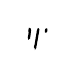
\begin{tikzpicture}
\begin{scope}[scale=0.015,yscale=-1]
%These are svgs of the 3 hebrew letters from wikipedia with the starting point modified.
  \filldraw svg{m136,549c-10.9-4.33-11.9-16.2-9.83-28.4,2.53-14.7,7.93-26.7,9.68-42,4.91-42.8,18.9-94.2,5.15-136,0-13.6-0.934-32,10.4-41.2,22.2-5.69,22.6-2.65,24.9,11.7,2.18,13.7,1.91,28.6,2.6,42.5-2.89,37.6-8.06,73.6-13.6,111-1.88,12.7-4.89,25.1-6.42,37.7-2.65,22,1.65,45-22.9,45z};
  \filldraw svg{m294.9,781c-12.8-6.42-18.7-20.8-20.8-34.3-0.548-3.39,0.711-4.58,3.54-11.4,6.85-16.6,6.53-26.5,13.1-47.6,4.94-16.5,9.12-45.5,13.3-77.1,8.38-64.1,17.1-116,29.4-179,4.92-25.3,9.13-54.5,6.58-60.7,0-19.6,3.55-51.8,23.6-61.8,7.92-3.95,8.68-1.7,11.9,5.97,1.33,3.17,2.41,6.57,3.67,9.76,0,18.9-3.06,37.9-6.59,56.9-4.74,25.6-8.99,50.7-14.5,76.1-17.1,79-21.6,149-39.6,229-3.72,16.4-9.65,30.5-9.59,47.2,0.0707,17.8-0.989,47.6-14,47.6z};
\filldraw svg{m541,387c-9-10-5-24-2-37 2-8 3-14 5-22 3-11 4-15 14-16 8-1 10-1 16,4 16,15 5,22-1,38-2,6-3,11-6,17-4,7-8,14-14,17-5,3-8,3-12-1z};
\end{scope}
\end{tikzpicture}
\fi
We therefore scale the character, preserving aspect ratio, to occupy a standard square, in particular $[-1,1]^2$.
This means that we will have no trouble with writers who chose to write in different sizes.

Small distortions in how a path looks are invariants for characters. Data augmentation is needed to take advantage of this, and doing so is needed to get good results on the CASIA data, but experimenting with augmentation is not my aim. I stick with a single method of augmentation which performs the following to each character, which works well, and which I inherited from Ben Graham.
The character is enlarged by a separate uniformly random factor in $[0.7,1.3]$ in the vertical and horizontal directions.
Then $\alpha$ is picked uniformly random in $[-0.3,0.3]$ and one of the following three things is picked to happen uniformly at random: (1) the character is rotated by $\alpha$ radians, (2) the character is horizontally sheered by $\alpha$, (3) the character is vertically sheered by $\alpha$. Then the character is scaled to lie within a fixed bounding box.
%function distortCharacter

\section{Chinese handwriting recognition results}
\label{sec:chinese}
Here I present some highlights of experiments attempting to learn the CASIA data with signatures and RNNs. 
The aim is to do well at this complex path classification task using a fast, smaller model.
A character is not a single path, it is a series of paths, one for each stroke. 
We come up with some way to use the signature to form a representation of a character which we feed to a traditional classifier.
Training as we did on a single desktop with a single graphics processing unit (GPU,\jind{GPU})\footnote{Originally designed for graphics, a piece of commodity hardware which is commonly and effectively used for training neural networks in addition to the central processing unit(s) (CPU\jind{CPU}) in each computer.} it is generally the case that the training time is dominated by the neural network operations on the GPU\@. 
Calculating minibatches with these representations on CPU-only background threads, for example using \ii, was fast enough that the GPU was continuously using the minibatches for training.
This indicates that further optimising the signature calculations would not significantly speed up this training.

\subsection{Signatures of each stroke}
The simplest method is to make a representation of each stroke and use the sequence of these representations as the input to the RNN\@. The signature alone would not make a good representation, as the network would not then have any indication of the relative locations of the strokes, which is important. We therefore use the starting point and the signature as the representation. We feed this to a  simple 1-layer LSTM, with the architecture shown in \autoref{fig:strokesig}. We trained the network with the common method Adam \cite{Adam} with its default parameters.

Because all the strokes are not much longer than a line in the bounding box, it was not necessary to normalise the signatures. In all these cases, the network was fully trained after 5 epochs which took about an hour. The final test accuracies are shown in \autoref{tab:strokesigres}. We see that the signature contains some useful information about the stroke. The method does not reach anywhere near useful accuracy.

\begin{figure}
\centering
%\begin{center}
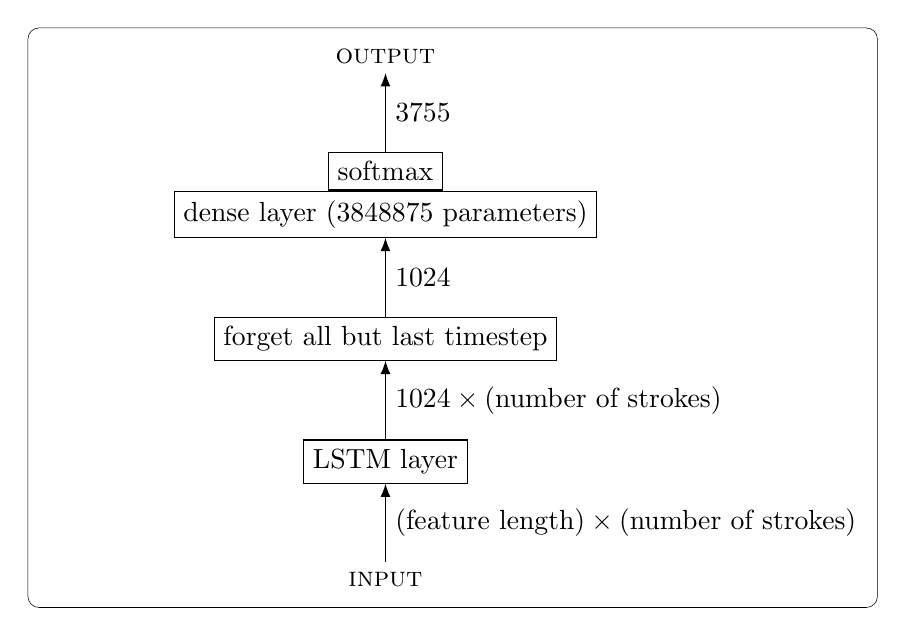
\begin{tikzpicture}[framed,background rectangle/.style={draw,very thin,rounded corners}]
\node (inp) {\textsc{input}};
\node[draw,rectangle,above =1 of inp] (l1) {LSTM layer};
%1081344 when level=2
%\node[above of = l1] (o1) {\rlap{\ $1024\times(\text{number of strokes})$}};
\node[draw,rectangle,above =1 of l1] (l3) {forget all but last timestep};
%\node[above of =l3] (o3) {\rlap{\ 1024}};
\node[draw,rectangle,above=1 of l3] (l4) {dense layer {\parameterSize(3848875 parameters)}};
\node[draw,rectangle,above=0 of l4] (s4) {softmax};
\node[above = 1 of s4] (o4) {\textsc{output}};
\draw[-Latex] (inp)--node[right](extreme){\parameterSize $(\text{feature length})\times (\text{number of strokes})$}(l1);
\draw[-Latex] (l1)--node[right]{\parameterSize $1024\times(\text{number of strokes})$}(l3);
\draw[-Latex] (l3)--node[right]{\parameterSize 1024}(l4);
\draw[-Latex] (s4)--node[right]{\parameterSize 3755}(o4);
%The next two lines are just to add space to the left of the diagram
%so that the main arrows are roughly in the middle
\coordinate (far left) at ($(extreme.east)!1.7!(l1)$);
\node at (far left) { };
\end{tikzpicture}
%\end{center}
\caption[Signatures of each stroke LSTM network schematic.]{\label{fig:strokesig}Schematic diagram of  LSTM network architecture for signatures of each stroke. The data shapes are indicated on the arrows.}%Numbers of parameters are indicated in circles.}
\end{figure}

%size of LSTM layer:
%def f(m,n):return 4*(n*m+n*n+n)
\begin{table}
\centering
%  \begin{center}
    \begin{tabular}{ccccc}
      \hline
      Signature level&representation length&Total parameters&test accuracy\\
      \hline
      none&2&8 055 467&0.267\\
      1&4&8 063 659&0.493\\
      2&8&8 080 043&0.576\\
      3&16&8 112 811&0.630\\
      4&32&8 178 347&0.658\\
      \hline
    \end{tabular}
%  \end{center}  
  \caption[Results for signatures of each stroke]{Results summary on CASIA1.1 of training LSTM on signatures of each stroke}
  \label{tab:strokesigres}
\end{table}


\subsection{Signatures of local segments}
This is a simple and more successful representation method of a character, which first converts the character to a single 3-dimensional path.
I discussed a few methods for making a single 3-dimensional path from a character in \cite{handwriting}. 
A basic method is to add a ``pen dimension'' which is 0 on each stroke (pen down) and 1 on an added straight line (pen up) between the endpoints of the strokes. 
These 3D paths vary in their total length. 
A  basic step is to chop the paths into segments of equal length. 
This length includes the length expended in the pen direction, otherwise the interpolation can produce weird artefacts. This makes it a bit more likely that a split in a path will happen at a pen lifting.
We experimented with overlapping the segments, but this was not clearly advantageous.
We use this split of the character as the time dimension of the RNN, picking some representation of each segment. 
Different characters will have different lengths, but the LSTM requires a whole minibatch to have the same time length, so we pad backwards in time with zeros.

A simple and effective representation is the starting point of the segment concatenated with the signature of the 3-dimensional path which is that segment up to some level.
We considered adding the bounding box or centroid of that segment but it did not obviously help.

In these comparisons, we split the characters into segments (after scaling) of length 0.4.
Different characters have different numbers of segments, with the maximum being around 115.
%On average, the number of segments is therefore %%%%%%%%%%
%Comparisons were made here using two LSTM layers of 512 units each, the Adam optimizer with the default parameters, which is joined to a single Dense layer. 
The architecture is %shown in \autoref{fig:logsigpen}.
just the same as for the signatures of strokes case, except the time dimension is now ``number of segments'' note ``number of strokes''.
%Because the paths have been normalised, we were able to do these experiments without scaling the inputs here.
Again, we used Adam with default parameters and we were able to do these experiments without scaling the inputs.
Beyond level 4 the representation of a character is far too large to learn from efficiently. Level 4 is already rather large.
We observe that this method is promising.

\iffalse
\begin{figure}
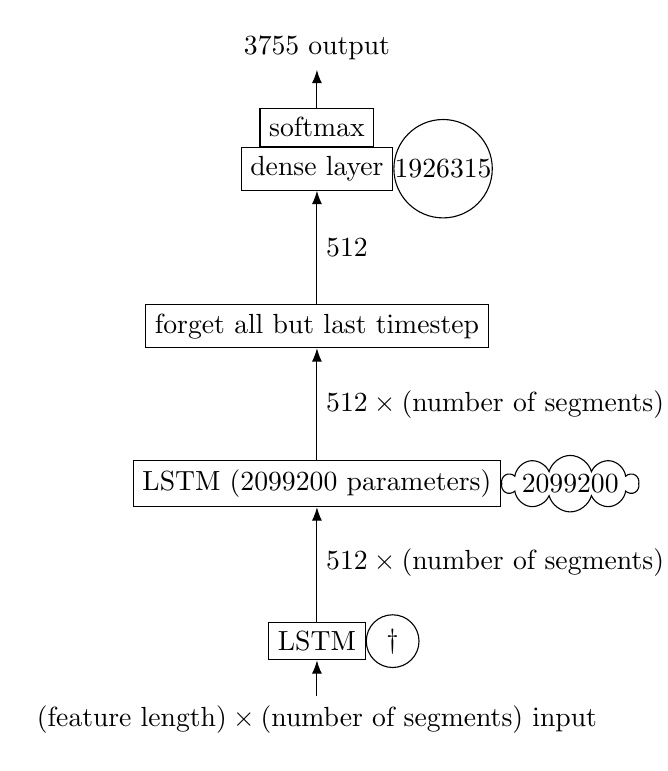
\begin{tikzpicture}
\node (inp) {$(\text{feature length})\times (\text{number of segments})$ input};
\node[draw,rectangle,above of=inp] (l1) {LSTM};
\node[draw,circle,right=0mm of l1] {$\dagger$};
%1081344 when level=2
\node[above of = l1] (o1) {\rlap{\ $512\times(\text{number of segments})$}};
\node[draw,rectangle,above of=o1] (l2) {LSTM (2099200 parameters)};
\node[draw,cloud ignores aspect,cloud,right=0mm of l2,inner sep=0mm] {2099200};
\node[above of = l2] (o2) {\rlap{\ $512\times(\text{number of segments})$}};
\node[draw,rectangle,above of=o2] (l3) {forget all but last timestep};
\node[above of =l3] (o3) {\rlap{\ 512}};
\node[draw,rectangle,above of=o3] (l4) {dense layer};
\node[draw,circle,right=0mm of l4,inner sep=0mm] {1926315};
\node[draw,rectangle,above=0mm of l4] (s4) {softmax};
\node[above of = s4] (o4) {3755 output};
\draw[-Latex] (inp)--(l1);
\draw[-Latex] (l1)--(l2);
\draw[-Latex] (l2)--(l3);
\draw[-Latex] (l3)--(l4);
\draw[-Latex] (s4)--(o4);
\end{tikzpicture}
\caption[Schematic diagram of  LSTM network architecture for signatures of local segments.]{\label{fig:logsigpen}Schematic diagram of  LSTM network architecture for signatures of local segments. 
Numbers of parameters are indicated in circles.}
\end{figure}
\fi
%2 512 layers
%m=2 5106859 totalparams

%now it's 1 layer with 1024 units
%m=1 have 
%m=2 have 4259840+3848875=8108715
%m=3 have 4370432+3848875=8219307

\begin{table}
\centering
%\begin{center}
    \begin{tabular}{ccccc}
      \hline
      Signature level&\multicolumn{1}{p{2.5cm}}{\centering representation length}&\multicolumn{1}{p{2cm}}{\centering Total parameters}&time (hr)&test accuracy\\
      \hline
      none&3  &8 059 563&14.9&0.909\\
      1   &6  &8 071 851&15.6&0.933\\
      2   &15 &8 108 715&15.6&0.945\\
      3   &42 &8 219 307&15.8&0.951\\
      4   &123&8 551 083&18.5&0.947\\
      \hline
    \end{tabular}
%  \end{center}  
  \caption[Results for signatures of local segments]{Results summary on CASIA1.1 of training LSTM on signatures of local segments. Training was for 10 epochs.}
  \label{tab:logsigpenres}
\end{table}
%Note to self: it's not stupid to include all 3 coordinates of the starting point of each
%segment. Some segments will begin with the pen up.

\section{Sketchnet}
\label{sec:sketch}
The Sketchnet dataset \cite{sketch} consists of hand-sketches of each of 250 classes of objects, like `tomato', `banana' and `TV' by 80 different writers. There is no standard train/test split, I take the first 40 of each for training and the last 40 for testing. This isn't comparable with others. 
Each stroke in the Sketchnet data is not given just as a series of points, but often includes a series of Bezier curves. The data thus appears to have been coarsened. I interpolate each given curve with ample points before doing anything else with the data, so that it is like the situation with CASIA data.

Unlike characters of handwriting, a flip in a vertical axis is a reasonable invariant for sketches and so I include such a flip with probability $\frac12$ in the data augmentation.

There has been much work on this type of human sketch recognition, most prominently Google's ``Quick, draw''\footnote{\url{https://quickdraw.withgoogle.com}} which went viral in 2017. The methods used were not released, but when I saw this work I knew they had much more data and much more accuracy than I could hope for.
Using a similar signatures of local segments method as for the RNNs with CASIA, and with very little tweaking, I got to a test error of 33\%.

\section{Signatures in LSTM}
\label{sec:lstmsig}
\def\inV{i}
\def\outV{f}
\def\inputindex{l}
Making models which are more efficient than LSTMs is something many people are trying.
LSTMs can take a long time to train, and although they perform very impressively they seem logically inefficient for a couple of reasons to my mind.\footnote{The thinking here is my woolly intuition, and is suffused with the traditional, perhaps lazy, anthropomorphism.}
First, that they have to learn these operations of ``whether to save'' and ``whether to forget'' individually, which is quite remote from the actual problem being solved.
Second, that if the thing they need to save is high dimensional they have to teach themselves into a state which allows a group of cells to cooperate.
We know that signatures provide a good summary of the shape of a path, and the history of something can sometimes be thought of as a path, and networks memory is just its choice of salient features of its memory, so we wondered whether we could  use signatures as this memory.
The signature would be an input to a cell of a RNN based on the history of that cell.
%Thinking about this is where the idea came from to somehow allow a signature of past start
Note in particular that \emph{this} effort is not trying to produce a network which is specially designed to handle curves or which is taking signatures of data as input, but rather we are trying to come up with something which solves the sort of problems a vanilla LSTM is used for, and is potentially a drop-in replacement, but is ultimately, hopefully, better in some way -- faster to train or smaller or more robust.
The signatures are taken internally in the network; the user would not need to know about them.
In this effort the derivatives of the signature are necessary because there are parameters in the calculation graph of the network which are affecting the input of signature calculations.
We tried several architectures to try to test out this type of idea, for example where a cell was given a signature of the graph of its activation through history as an input.

Only one type of architecture was successful in the most minimal way, namely that we could train the network to solve a toy problem.
This was suggested by Harald Oberhauser, and involves following the structure of the LSTM as closely as possible. 
For example, we want to separate the internal memory from the output of a layer, and we want to separate the space where the memory lives from the spaces of our layer's inputs and outputs.
The idea is that, for some $K$ and $m$, the memory is a signature of a $K$-dimensional path up to level $m$,
%The suggestion is to replace the memory cell with a signature - 
i.e.~a value in a truncated tensor space $T^{\underline m}(\mathbb{R}^K)$. We are not defining it by specifying the path of which it is the signature. We choose a configuration which will be the same as vanilla LSTM when $m=1$ but generalises it for $m>1$.

The way we forget is to collapse the signature in a chosen direction, either entirely or partially. The matrix of stretching by a factor $\lambda$ in the direction of the unit vector $\hat \inV$ is $(I_K-(1-\lambda)\hat \inV\hat \inV^T)$.
% and we apply this transformation to the signature by premultiplying each level $m$ by its $m$th Kronecker-product power. %the iterated Kronecker product $(I_K+(\lambda-1)\vec a\vec a^T)^{\otimes m}$. 
If we were to generate $\hat\inV$ on its own in the network by making a vector $\vec \inV$ and normalising it there would be a nasty discontinuity around small $\vec \inV$. It would be nicer to do something like using $\|\vec \inV\|$ to get $1-\lambda$ or (which looks nicer) $\sqrt{1-\lambda}$ so that small values of $\vec \inV$ don't do anything. But we don't want $1-\lambda$ to be bigger than 1. So we use $\tanh \|\vec \inV\|$ as $\sqrt{1-\lambda}$ to get the matrix $\left(I_K-\frac{\tanh^2\|\vec \inV\|}{\|\vec \inV\|^2}\vec \inV\vec \inV^T\right)$.
%Call this operation on signatures $\text{Forget'}_{\lambda,\vec a}(\cdot)$.
To apply this transformation to the signature we premultiply each level $m'$ by the matrix's $m'$th Kronecker-product power. Call $\vec \inV$ the \emph{forget-vector}, and this operation on signatures $\text{Forget}_{\vec \inV}(\cdot)$.\footnote{In practice, this uses the \texttt{sigscale} functionality of \ii.}

To save information, we concatenate a new segment onto the path -- i.e.~Chen product the stored signature with the signature of a chosen segment.\footnote{In practice, this uses the \texttt{sigjoin} functionality of \ii.} %I use $\otimes$ to represent the Chen product. 
We need to pick the new segment in a sensible way to maintain the scaling of the signature, so we always make the new segment be a unit vector. %Just picking a unit vector would do, but I think we also had simpler ideas for this when we spoke in Oxford -- I think one was making $K$ equal to $L$ and just using the inputs. So 
We let $\text{Add}_{\vec \outV}(S)$ be the signature obtained as the Chen product of $S$ and $\exp (\frac1{\|\vec \outV\|}\vec \outV)$

We call one of these stored signatures a \emph{signature cell}. There are clearly many variations which could be tried, but for these experiments we have only one of them in the whole layer. We call the number of hidden units in the layer $u_{i+1}^0$. %$P$
%, we have a choice about how to group them - should there be more than one of them  - having only one isn't stupid, they can store lots of information. For the moment, let's say there are $N$ of them (labelled with $n$), and they all have the same number $K$ of dimensions (labelled with $k$) and maximum level $M$. Let the signature cell have value $S_{nt}$. Let each signature cell have $P$ hidden units (labelled with $p$).

We can't have an equation like \eqref{eq:forget} for a signature cell because a linear combination of signatures doesn't produce a signature. A simple way to do some forgetting and adding is to always do the forgetting and then always concatenate something on.

How to generate output based on the signature -- in analogy with (\ref*{eq:output}) -- is not obvious. Having a parameter the shape of a signature and using it as a linear functional is out solution to this, although it does involve adding many extra parameters.

Putting things together, we have the following parameters for an input to our layer $i$ of shape $u_i^0\times u_i^1$. $K\times u_i^1$ weights matrices $W^f$ and $W^i$, $K\times u_{i+1}^0$ weights matrices $\bar W^f$ and $\bar W^i$, and length-$K$ biases $b^f$ and $b^i$. $u_{i+1}^0\times u_i^1$ weights matrix $W^o$, $u_{i+1}^0\times u_{i+1}^0$ weights matrix $\bar W^o$, and length-$u_{i+1}^0$ biases $b^o$ and $b^h$ (if $S$ doesn't include a fixed 1). Also $u_{i+1}^0$ signature-shaped parameters $V^h$ each of size $\frac{u_{i+1}^0((u_{i+1}^0)^m-1)}{u_{i+1}^0-1}$ -- another big matrix. 
We used a common scheme for initialising the parameters -- the biases were initialised at zero, and each weight matrix was initialised in the ``Glorot Uniform'' method built in to Keras -- each element being uniformly distributed in $[-\frac{\sqrt 6}{g},\frac{\sqrt 6}{g}]$ where $g$ is the sum of the matrix's last two dimensions. The following are the complete defining equations, note that the variables $p$ and $p'$ vary among the $u_{i+1}^0$ output units.
\begin{align}
\inV_{kt}&=\sum_\inputindex W^\inV_{k\inputindex} ((g_i)_t)_\inputindex+\sum_{p'} \bar W^\inV_{kp'}h_{p',t-1}+b^\inV_{k}&&\text{\parbox{1.4in}{\raggedright $k$th element of forget vector $\vec \inV_{t}$}}\\
\outV_{kt}&=\sum_\inputindex W^\outV_{k\inputindex} ((g_i)_t)_\inputindex+\sum_{p'} \bar W^\outV_{kp'}h_{p',t-1}+b^\outV_{k}&&\text{\parbox{1.4in}{\raggedright $k$th element of new information vector $\vec \outV_{t}$}}\\
o_{pt}&=\sigma\left(\sum_\inputindex W^o_{p\inputindex} ((g_i)_t)_\inputindex+\sum_{p'} \bar W^o_{pp'}h_{p',t-1}+b^o_{p}\right)&&\text{\parbox{1.4in}{\raggedright in [0,1], whether to output anything}}\\
S_{t}&=\text{Add}_{\vec \outV_{t}}(\text{Forget}_{\vec \inV_{t}}(S_{t-1}))\\
\tilde h_{pt}&=V^h_{p}\cdot S_{t}+b^h_{p}&&\text{\parbox{1.4in}{\raggedright\setstretch{1} dot product of signatures as potential output}}\\
h_{pt}&=o_{jt}\tanh(\tilde h_{pt})&&\text{output}
\end{align}
The structure of a single timestep of one of these LSTM signature layers is summarised in \autoref{fig:LSTMsig}.
\begin{figure}
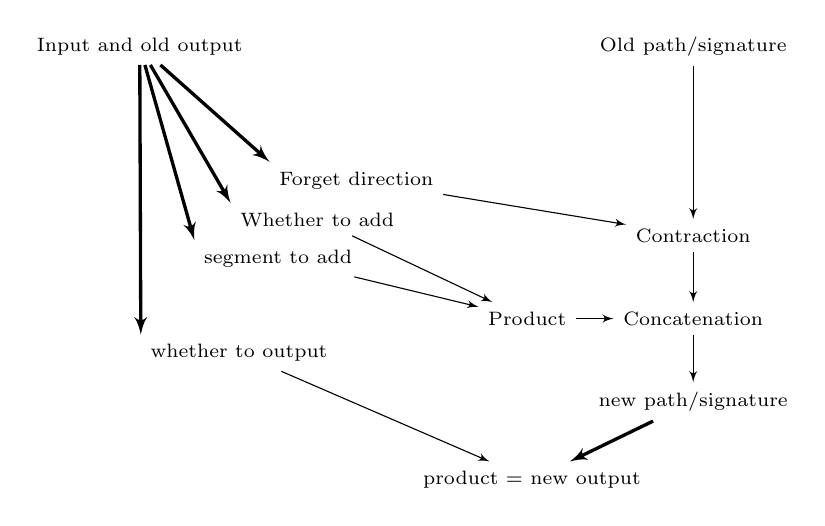
\begin{tikzpicture}[font=\scriptsize,node distance=2.4cm,auto]
	\node(a) {Input and old output};
	\node(aa) [xshift=20em]{Old path/signature};
	\node(b) [below right of=a,text centered,xshift=3em]{Forget direction};
	\node(w) [below left of=b,text centered,node distance=2em]{Whether to add};
	\node(s) [below left of=w,text centered,node distance=2em]{segment to add};
	\node(ww) [below left of=s,text centered,node distance=2em,yshift=-2em]{whether to output};
	\node(c) [below of=aa]{Contraction};
	\node(cc) [below of=c,node distance=3em]{Concatenation};
	\node(p) [left of=cc,node distance=6em]{Product};
	\node(nps) [below of=cc,node distance=3em]{new path/signature};
	\node(out) [below left of=nps,xshift=-3em,node distance=4em]{product = new output};
	\draw[-latex',very thick] (a) -> (b.north west);
	\draw[-latex',very thick] (a) -> (w.north west);
	\draw[-latex',very thick] (a) -> (s.north west);
	\draw[-latex',very thick] (a) -> (ww.north west);
	\draw[-latex'] (b) -> (c);
	\draw[-latex'] (aa) -> (c);
	\draw[-latex'] (c) -> (cc);
	\draw[-latex'] (w) -> (p);
	\draw[-latex'] (s) -> (p);
	\draw[-latex'] (p) -> (cc);
	\draw[-latex'] (cc) -> (nps);
	\draw[-latex'] (ww) -> (out);
	\draw[-latex',very thick] (nps) -> (out);
	\end{tikzpicture} 
\caption[Schematic of one cell of an LSTM layer with signature memory.]{\label{fig:LSTMsig}Schematic of one cell of an LSTM layer with signature memory. Bold arrows indicate that learned parameters are involved.}
\end{figure}


\subsection{Toy problem}
We wanted a very simple example problem to see if our new design of network could (a) learn anything and (b) have memory, i.e.~learn something which depends only on a long-term dependency in the data. We wanted the problem to be simple as the calculation is quite slow despite using \ii, because significantly it is happening on a CPU rather than a GPU\@. We came up with the following task, which  can also easily be solved with a traditional LSTM\@. The task is to distinguish between (category $A$) a random binary string of i.i.d.~Bernouilli$(0.5)$ zeros and ones, and (category $B$) a string which begins with a shorter length $v$ binary string and continues with the length $v$ partial sums mod 2. For example, the following are such strings with $v=4$.
\begin{align*}
0010\ 1001001001\\
1011\ 1101111011
\end{align*}
Distinguishing these requires remembering something for at least $v$ steps. 
Also it is not possible to distinguish the classes perfectly, because a random string may have the form of the other strings by chance, but this is a small effect.
For the experiments I had a single one of my LSTM-signature layers, of which the value of the timestep was passed to a dense layer with 40 ReLU units, which was connected to a single sigmoid output. A summary of the network in use is shown in \autoref{fig:toyLSTM}.
\begin{figure}
\centering
%\begin{center}
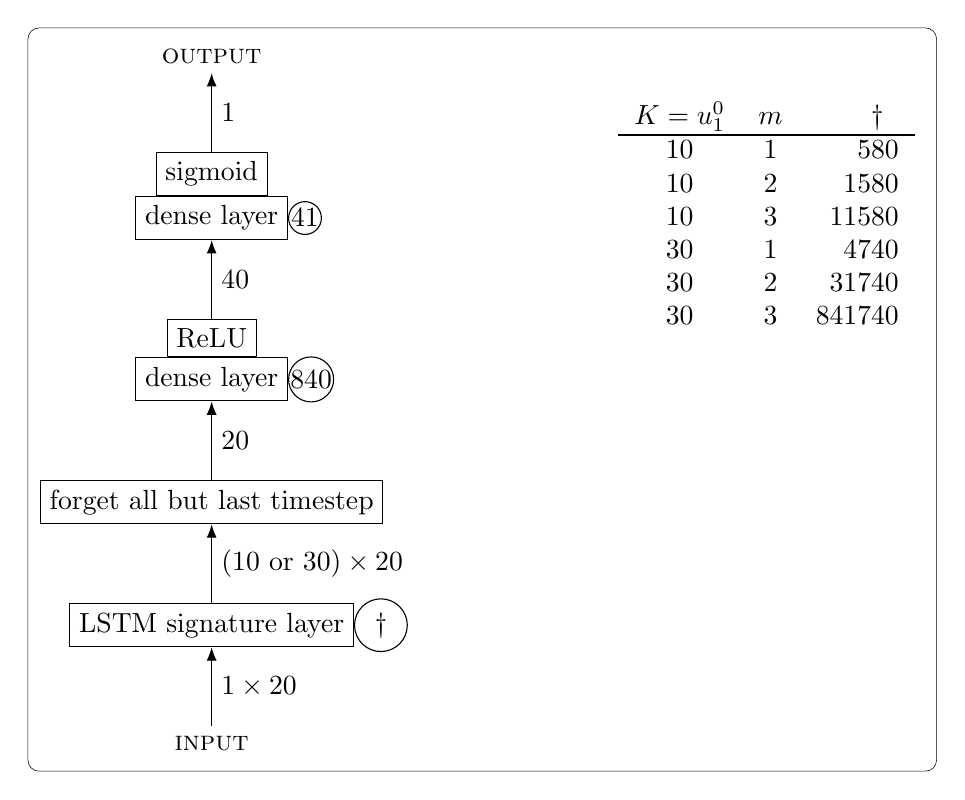
\begin{tikzpicture}[framed,background rectangle/.style={draw,very thin,rounded corners}]
\node (inp) {\textsc{input}};
\node[draw,rectangle,above =1 of inp] (l1) {LSTM signature layer};
\node[draw,circle,right=0mm of l1] {$\dagger$};
%\node[above of = l1] (o1) {\rlap{\ $(10\text{ or }30)\times20$}};
\node[draw,rectangle,above=1 of l1] (l2) {forget all but last timestep};
%\node[above of = l2] (o2) {\rlap{\ 20}};
\node[draw,rectangle,above=1 of l2] (l3) {dense layer};
\node[draw,circle,right=0mm of l3,inner sep=0mm] {840};
\node[draw,rectangle,above=0mm of l3] (s3) {ReLU};
%\node[above of =s3] (o3) {\rlap{\ 40}};
\node[draw,rectangle,above=1 of s3] (l4) {dense layer};
\node[draw,circle,right=0mm of l4,inner sep=0mm] {41};
\node[draw,rectangle,above=0mm of l4] (s4) {sigmoid};
\node[above = 1 of s4] (o4) {\textsc{output}};
\draw[-Latex] (inp)--node[right]{\parameterSize $1\times20$}(l1);
\draw[-Latex] (l1)--node[right]{\parameterSize $(10\text{ or }30)\times20$}(l2);
\draw[-Latex] (l2)--node[right]{\parameterSize 20}(l3);
\draw[-Latex] (s3)--node[right]{\parameterSize 40}(l4);
\draw[-Latex] (s4)--node[right]{\parameterSize 1}(o4);
\node[right=1.6in of l4]{
  \begin{tabular}{ccr}
$K=u_1^0$&$m$&$\dagger\;\;$\\
\hline
10&1&580\\
10&2&1580\\
10&3&11580\\
30&1&4740\\
30&2&31740\\
30&3&841740
  \end{tabular}
};
\end{tikzpicture}
%\end{center}
\caption[LSTM signature schematic]{\label{fig:toyLSTM}Schematic diagram of architecture used for training an LSTM signature layer on a toy model. 
The data shapes are indicated on the arrows. 
Numbers of parameters are indicated in circles.}
\end{figure}

Because this was just a proof-of-concept and unlimited data could be generated, there was no need to have separate train and test sets. We just had a very large training set, which is highly representative of the two classes. The general result was that these networks were able to learn, but took a long time to start learning in some cases. This 
seems to be because initialisation is hard to get right. 
The graphs show the accuracy over the whole training set of 11000 samples after each epoch (pass through the whole of the data).
In the experiments which I plotted, $v$ is 15 and so 15 of the $u_0=20$ units are always random, so it is not easy to memorise the members of category $B$ and memory of length 15 steps is requires.
In \autoref{fig:lstmsig201010} I show cases for $m=1,2,3$ for $K=u_1^0=10$, and in \autoref{fig:lstmsig203030} I show cases for $K=u_1^0=30$.

        \begin{figure}
	\includegraphics[width=0.85\textwidth]{lstmsig20_10_10}
          \caption[LSTM Signature training accuracy -- 10D with 10 hidden units]{Accuracy of the classification of training the LSTM Signature network on the toy problem after each epoch. The first 15 of the 20 characters are random. Signature level: blue 1, red 2, yellow 3. 10 dimensions with 10 hidden units.}
          \label{fig:lstmsig201010}
        \end{figure}
        \begin{figure}
	\includegraphics[width=0.85\textwidth]{lstmsig20_30_30}
          \caption[LSTM Signature training accuracy -- 30D with 30 hidden units]{Accuracy of the classification of training the LSTM Signature network on the toy problem after each epoch. 15 of the 20 characters are random. Signature level: blue 1, red 2, yellow 3. 30 dimensions with 30 hidden units.}
          \label{fig:lstmsig203030}
        \end{figure}

There is a lot of scope for playing with this model --- many parameters to tweak and various initialisations to try. If investing heavily into this, I would want to move the calculations onto a GPU for much more efficiency, and then try to learn a standard sequence modelling benchmark, such as the famous Penn Treebank. The success of this experiment is in showing that something can be learnt by a layer with a signature inside.
\endDocumentJR
